\documentclass[11pt]{article}

\usepackage{fullpage}
\usepackage{graphicx}
\usepackage{amsmath}
\usepackage{amssymb}
\usepackage{amsthm}
\usepackage{fancyvrb}

\parindent0in
\pagestyle{plain}
\thispagestyle{plain}

\newcommand{\myname}{Mehshan Mustafa}
\newcommand{\dated}{\today}

\newenvironment{theorem}[2][Theorem]{\begin{trivlist}
\item[\hskip \labelsep {\bfseries #1}\hskip \labelsep {\bfseries #2.}]}{\end{trivlist}}
\newenvironment{lemma}[2][Lemma]{\begin{trivlist}
\item[\hskip \labelsep {\bfseries #1}\hskip \labelsep {\bfseries #2.}]}{\end{trivlist}}
\newenvironment{exercise}[2][Exercise]{\begin{trivlist}
\item[\hskip \labelsep {\bfseries #1}\hskip \labelsep {\bfseries #2.}]}{\end{trivlist}}
\newenvironment{problem}[2][Problem]{\begin{trivlist}
\item[\hskip \labelsep {\bfseries #1}\hskip \labelsep {\bfseries #2.}]}{\end{trivlist}}
\newenvironment{question}[2][Question]{\begin{trivlist}
\item[\hskip \labelsep {\bfseries #1}\hskip \labelsep {\bfseries #2.}]}{\end{trivlist}}
\newenvironment{corollary}[2][Corollary]{\begin{trivlist}
\item[\hskip \labelsep {\bfseries #1}\hskip \labelsep {\bfseries #2.}]}{\end{trivlist}}
\newenvironment{solution}{\begin{proof}[Solution]}{\end{proof}}
\newenvironment{idea}[2][Proof Idea.]{\textit{#1} #2}

\begin{document}

\textbf{Introduction to the Theory of
Computation}\hfill\textbf{\myname}\\[0.01in]
\textbf{Chapter 1: Reqular Languages}\hfill\textbf{\dated}\\
\smallskip\hrule\bigskip

\begin{problem}{1.71}
Let $\Sigma = {0, 1}$.
\end{problem}

\begin{problem}[Part]{a}
Let $A = \{0^{k}u0^{k} \; | \; k \geq 1 \; and \; u \in \Sigma^{*}\}$. Show that A is regular.
\end{problem}

\begin{idea}
State diagram of an NFA that recognizes $A_{k=2}$.
\begin{center}
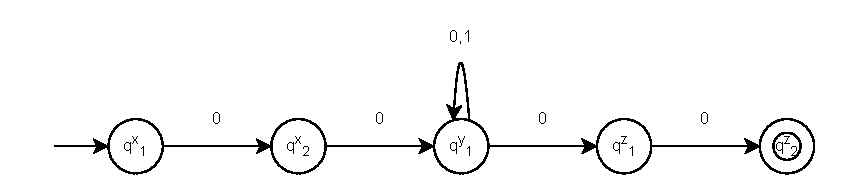
\includegraphics[scale=1.0]{Figures/Problem1.71.pdf}
\end{center}
\end{idea}

\begin{proof}
The proof is by construction.
Construct the NFA $N = (Q, \; \Sigma, \; \delta, \; q_{0}, \; F)$ that recognizes $A$:
\begin{enumerate}
\item $Q = Q^x \cup Q^y \cup Q^z$, where:
\[ Q^x = \{q_{1}^x, \; q_{2}^x, \; q_{3}^x, \; \cdots, \; q_{k}^x\} \]
\[ Q^y = \{q_{1}^y\} \]
\[ Q^z = \{q_{1}^z, \; q_{2}^z, \; q_{3}^z, \; \cdots, \; q_{k}^z\} \]
\item $q_{0} = q_{1}^a$
\item $F = \{q_{k}^c\}$
\item Define $\delta$ so that for any $q_{i}^u \in Q$ and any $a \in \Sigma$:
\end{enumerate}
\begin{center}
$\displaystyle \delta(q_{i}^u,\ a) \ =\begin{cases}
\{q_{i+1}^x\} & u=x \ ,\ i<k \ and \ a = 0 \\
\{q_{1}^y\} & u=x \ , \ i=k \ and \ a = 0 \\
\{q_{1}^y, \ q_{1}^z\} & u=y \ , \ i=1 \ and \ a = 0 \\
\{q_{1}^y\} & u=y \ , \ i=1 \ and \ a = 1 \\
\{q_{i+1}^z\} & u=z \ ,\ i<k \ and \ a = 0 \\
\phi & u=z \ ,\ i=k
\end{cases} \ \ $
\end{center}
\end{proof}

\begin{problem}[Part]{b}
Let $B = \{0^{k}1u0^{k} \; | \; k \geq 1 \; and \; u \in \Sigma^{*}\}$. Show that B is not regular.
\end{problem}

\begin{proof}
Solution Replace this text with the details of your proof or solution.
\end{proof}

\end{document}